\documentclass[a4paper]{article}
% \pagestyle{empty}

\title{Progetto finale Reti Logiche}
\author{Luca De Martini}
\date{}

\usepackage[a4paper,width=150mm,top=20mm,bottom=20mm]{geometry}
% \usepackage[hidelinks]{hyperref}
\usepackage[table]{xcolor}
\usepackage{wrapfig}
\usepackage{array,multicol,graphicx,multirow,float}
\usepackage[activate=true,final,tracking=true,kerning=true,spacing=true]{microtype}
\microtypecontext{spacing=nonfrench}


\begin{document}

\setlength\parindent{0pt}
% \hyphenpenalty=1500
\emergencystretch 3em

\begin{figure}[t]
  
\includegraphics[height=3cm]{logoPoli.pdf}
\end{figure}

\maketitle

\section{Introduzione}

Il componente realizzato implementa la codifica ``Working Zone'' per indirizzi di 7 bit con 8 working zones di dimensione 4.

La codifica working zone consiste nell'esprimere un indirizzo in funzione della sua posizione relativa all'inizio di una working zone, se ne fa parte, altrimenti lasciarlo invariato.

Se l'indirizzo da codificare non fa parte di nessuna working zone il primo bit viene messo a `0' e i restanti 7 bit sono quelli dell'indirizzo invariato.

Per un indirizzo che fa parte di una working zone il risultato è composto da tre parti: il primo bit messo a `1' a indicare che l'indirizzo fa parte di una working zone, i successivi 3 bit contengono il numero della working zone in cui rientra l'indirizzo espresso in codifica binaria (da 000 a 111), mentre gli ultimi 4 bit contengono l'offset dell'indirizzo rispetto all'inizio (o base) della working zone espresso in codifica one-hot (da 0001 a 1000)

In tabella \ref{tab:example} sono riportati degli esempi di codifica, dove l'indirizzo codificato è separato a indicare le diverse parti del risultato.

\begin{table}[H]
  \centering
  \ttfamily
  \begin{tabular} {|c|c|c|}
    \hline
    \bf{Address} & \bf{Working zones}          & \bf{Encoded address} \\
    \hline
    ...          &                             & ...                  \\
    \hline
    0000110      &                             & 0 0000110            \\
    \hline
    0000111      & \cellcolor[HTML]{E0E0E0}wz2 & 1 010 0001           \\
    \hline
    0001000      & \cellcolor[HTML]{E0E0E0}wz2 & 1 010 0010           \\
    \hline
    0001001      & \cellcolor[HTML]{E0E0E0}wz2 & 1 010 0100           \\
    \hline
    0001010      & \cellcolor[HTML]{E0E0E0}wz2 & 1 010 1000           \\
    \hline
    0001011      &                             & 0 0001011            \\
    \hline
    0001100      &                             & 0 0001100            \\
    \hline
    0001101      &                             & 0 0001101            \\
    \hline
    0001110      & \cellcolor[HTML]{E0E0E0}wz3 & 1 100 0001           \\
    \hline
    ...          & \cellcolor[HTML]{E0E0E0}wz3 & ...                  \\
    \hline
  \end{tabular}
  
  wz2 = 0000111, wz3 = 0001110
  \caption{Esempio di codifica}
  \label{tab:example}
\end{table}

\pagebreak
\section{Architettura}
Al livello più alto il componente presenta un modulo \texttt{project\_reti\_logiche} che contiene tutti i moduli interni, un'automa a stati finiti e un registro di cache dell'indirizzo in output.

\begin{figure}[H]
  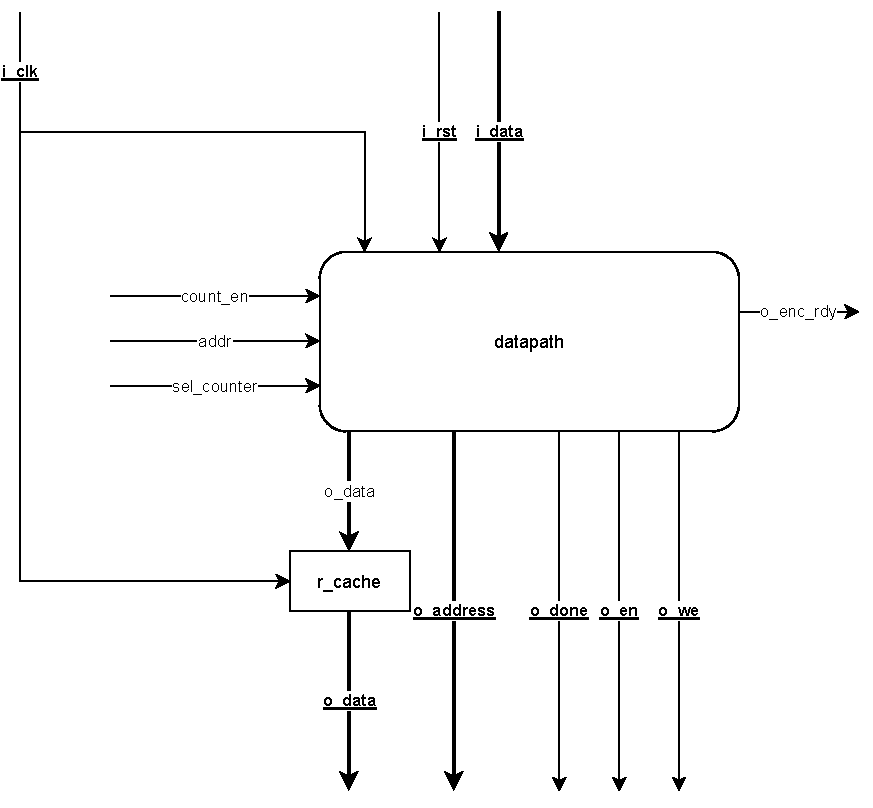
\includegraphics[width=12cm]{schema-main.pdf}
  \caption{Schema modulo principale}
  \label{fig:schema}
\end{figure}

L'automa a stati finiti è implementato con una collezione di process:

Due process descrivono il comportamento del registro di cache e quello del registro di stato, entrambi sono realizzati con flip-flop sincroni attivati sul fronte di discesa, la scelta di usare il falling edge è stata fatta per ridurre il numero di cicli di clock necessari per la codifica.

Un altro process aggiorna il valore del segnale \texttt{next\_state} in base allo stato attuale, al segnale in input di \texttt{i\_start} e al segnale \texttt{enc\_rdy}, output del modulo interno \texttt{datapath} che verrà descritto nel dettaglio successivamente.

Infine un ultimo process aggiorna i valori dei segnali in input ai moduli interni e in output dal componente necessari al funzionamento basandosi sullo stato attuale.

\begin{figure}[H]
  \centering
  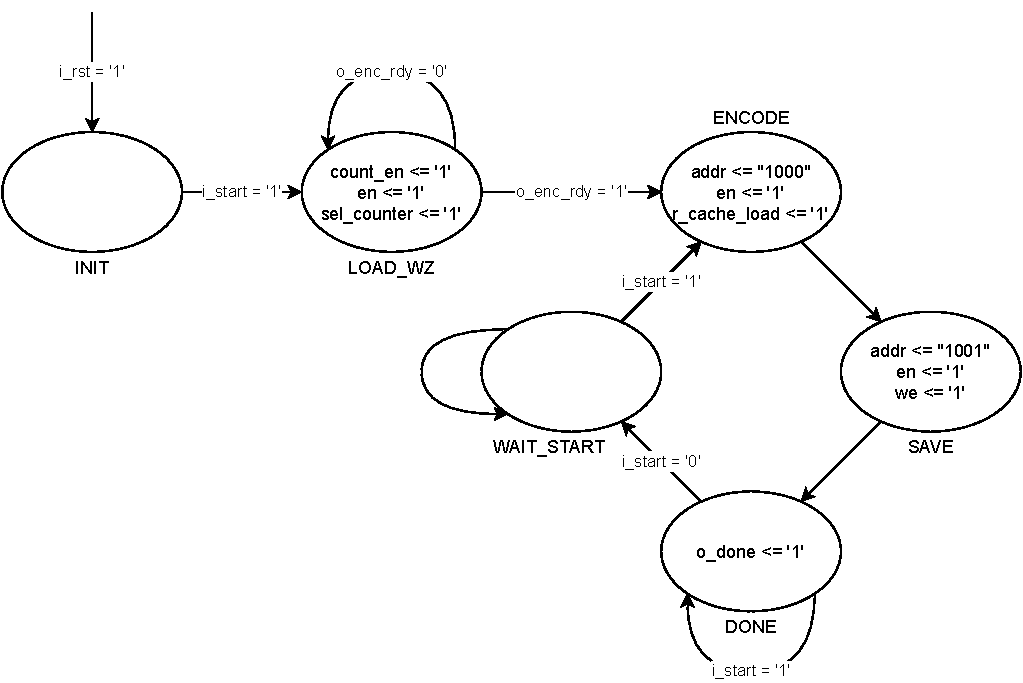
\includegraphics[width=12.5cm]{schema-fsa.pdf}
  \caption{Automa a stati finiti}
  \label{fig:fsa}
\end{figure}

L'FSA ha 6 stati ed è caratterizzato da due zone di funzionamento, la prima zona è quella iniziale di setup costituita dagli stati `INIT' e `LOAD\_WZ': una volta ricevuto il segnale di \texttt{i\_start} il componente si prepara alla codifica rimanendo nello stato `LOAD\_WZ' mentre sta caricando gli indirizzi delle working zones nei suoi registri interni.

La fine di questa fase è segnalata dal segnale \texttt{o\_enc\_rdy} proveniente dai componenti interni che viene alzato a `1' quando è pronto a codificare, avanzando così l'automa al prossimo stato `ENCODE' e iniziando la fase di codifica.

La fase di codifica iniza nello stato `ENCODE' dove il componente legge l'indirizzo da codificare, lo codifica e lo carica nel registro di cache in un unico ciclo di clock. Nello stato seguente, `SAVE', viene scritto in RAM il risultato e in quello dopo, `DONE', viene alzato il segnale di \texttt{o\_done} segnando la fine della codifica.

Dopo di che il componente attenderà l'abbassarsi del segnale di \texttt{i\_start} per abbassare \texttt{o\_done} e poi mettersi in attesa di un nuovo segnale di start nello stato `WAIT\_START', pronto per una nuova codifica.

\pagebreak
\subsection{Moduli interni}

\begin{wrapfigure}[14cm]{R}{3.5cm}
  \centering
  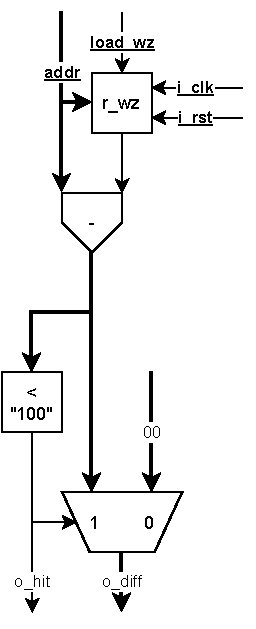
\includegraphics[width=3.5cm]{schema-wz_enc.pdf}
  \caption{Schema di \texttt{wz\_enc}}
  \label{fig:wz_enc}
\end{wrapfigure}

\begin{figure}[H]
  \centering
  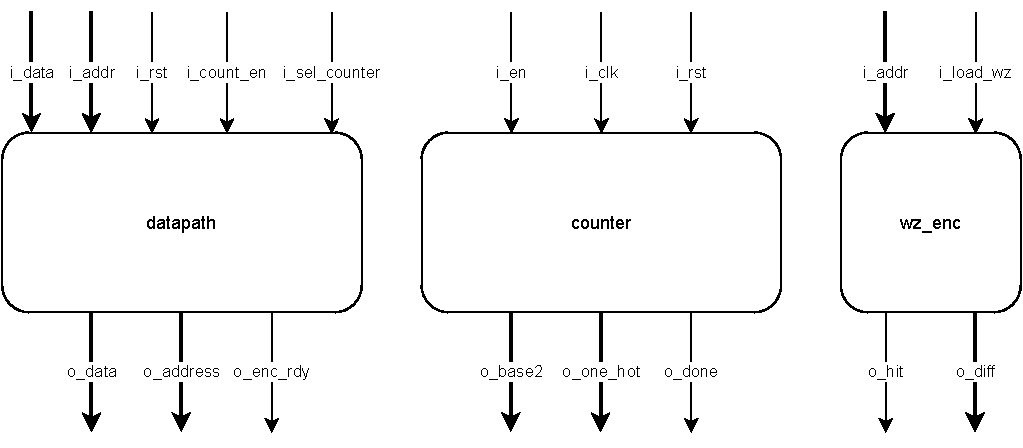
\includegraphics[width=10cm]{schema-components.pdf}
  \caption{Moduli interni}
  \label{fig:modules}
\end{figure}

Il componente contiene un modulo \texttt{datapath} che ha al suo interno un modulo \texttt{counter} e 8 moduli \texttt{wz\_enc} identici (uno per ogni indirizzo della working zone).

\subsubsection{wz\_enc}

I moduli \texttt{wz\_enc} si occupano di stabilire se un indirizzo sia all'interno di una determinata working zone, segnalandolo con \texttt{o\_hit}, e di calcolarne l'offset in caso positivo. L'offest rispetto alla working zone è \texttt{o\_diff} che è da considerarsi valido solo se \texttt{o\_hit} è a `1', altrimenti avrà tutti i bit a `0'

\subsubsection{counter}

Il modulo \texttt{counter} è un contatore da 0 a 7 che scatta sul falling edge. Esso inizia a contare quando riceve un segnale di enable, dando l'output sia in codifica binaria, sia in codifica one hot, dopo aver sorpassato il 7 tutti i bit degli output vengono messi a `0'

\subsubsection{datapath}

\begin{figure}[H]
  \centering
  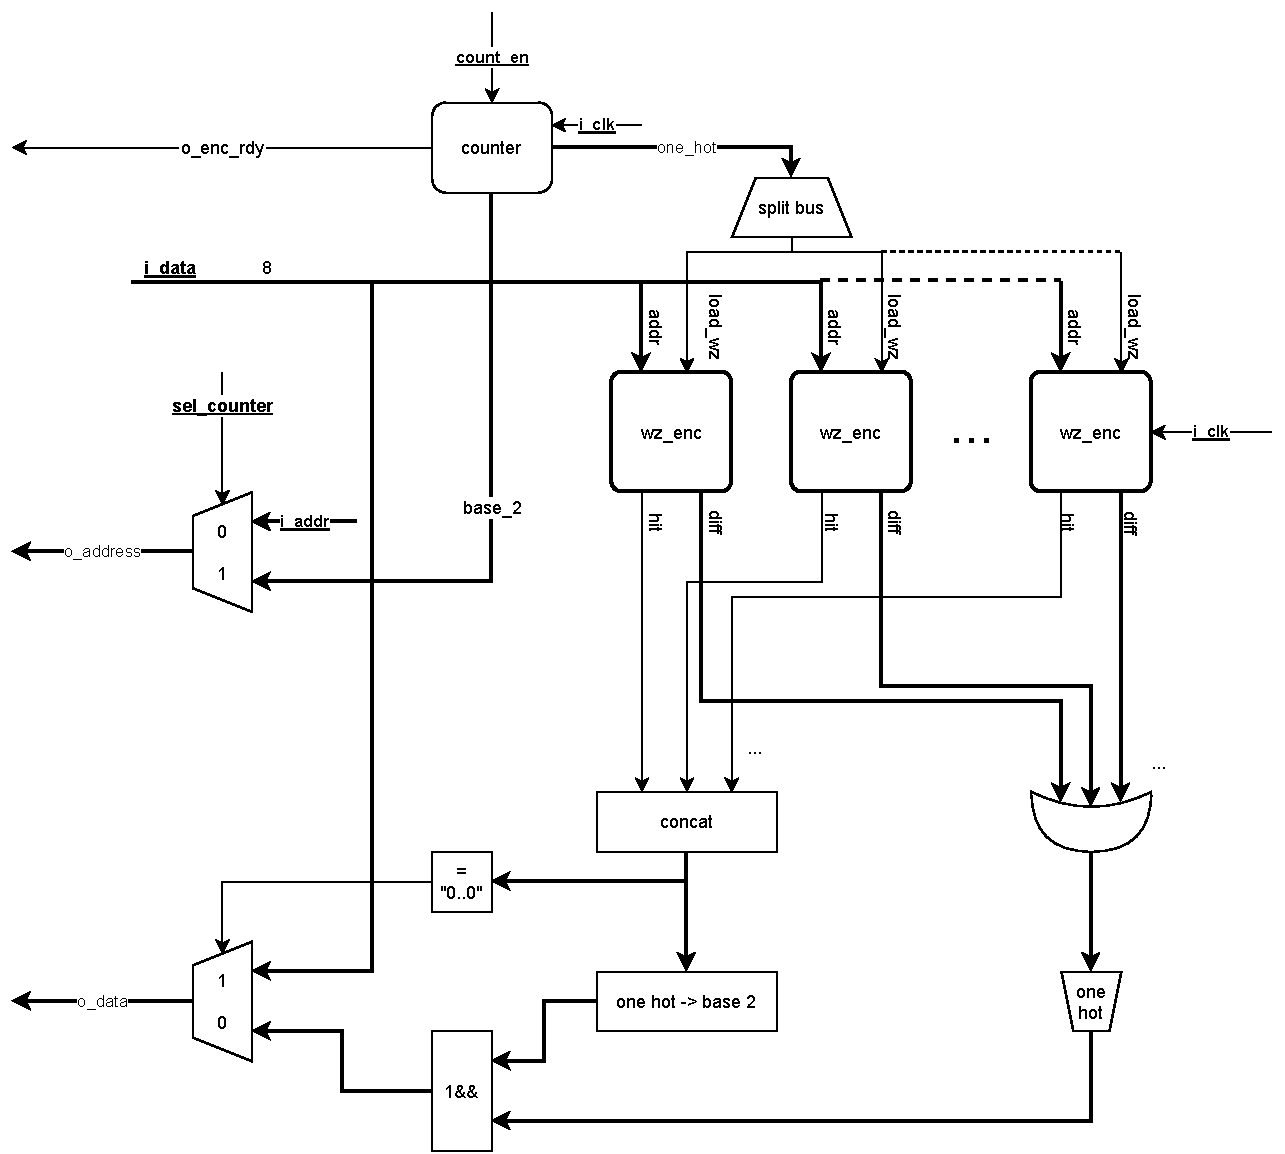
\includegraphics[width=\linewidth]{schema-datapath.pdf}
  \caption{Schema di \texttt{datapath}}
  \label{fig:datapath}
\end{figure}

Il \texttt{datapath} divide il bus contenente la codifica one hot in uscita dal \texttt{counter} collegando ogni bit del segnale al segnale di load di un \texttt{wz\_enc}, in questo modo, usando il segnale in codifica binaria per l'indirizzo in uscita permette di caricare l'indirizzo delle working zone nei rispettivi registri. 

Utilizzando l'output degli \texttt{o\_hit} dei \texttt{wz\_enc} il \texttt{datapath} può rilevare se un indirizzo faccia parte di una working zone o meno, poi combinando gli output degli \texttt{o\_diff} può calcolare la codifica completa dell'indirizzo.


\section{Risultati sperimentali}

Dal report di sintesi si può osservare che il design del componente utilizza in minima parte le risorse disponibili sulla superficie dell'FPGA, non sono presenti black-box e non sono state sintetizzate strutture con un numero di componenti indesiderato.

\hspace{8em}
\begin{table}[H]
  \centering
  \begin{tabular}{|p{3.5cm}|c|c|}
    \hline
    \bf{Site Type}        & \bf{Used} & \bf{Util\%} \\
    \hline
    Slice LUTs*           & 98        & 0.07        \\
    \hline
    LUT as Logic          & 98        & 0.07        \\
    \hline
    LUT as Memory         & 0         & 0.00        \\
    \hline
    Slice Registers       & 71        & 0.03        \\
    \hline
    Register as Flip Flop & 71        & 0.03        \\
    \hline
    Register as Latch     & 0         & 0.00        \\
    \hline
  \end{tabular}
  \caption{Slice Logic}
\end{table}

\hspace{8em}

Il numero di nodi utilizzato scala linearmente con il numero di working zone e visto l'ampio margine disponibile sarebbe possibile creare un componente che supporti più working zones con questo stesso design senza incorrere in problemi di eccessiva utilizzazione della superficie dell'FPGA

\hspace{8em}
\begin{table}[H]
  \centering
  \begin{tabular}{|p{2cm}|c|p{3.70cm}|}
    \hline
    \bf{Ref Name} & \bf{Used} & \bf{Functional Category} \\
    \hline
    FDRE          & 71        & Flop \& Latch            \\
    \hline
    LUT2          & 58        & LUT                      \\
    \hline
    OBUF          & 27        & IO                       \\
    \hline
    LUT4          & 16        & LUT                      \\
    \hline
    CARRY4        & 16        & CarryLogic               \\
    \hline
    LUT5          & 15        & LUT                      \\
    \hline
    LUT6          & 13        & LUT                      \\
    \hline
    IBUF          & 11        & IO                       \\
    \hline
    LUT3          & 7         & LUT                      \\
    \hline
    LUT1          & 1         & LUT                      \\
    \hline
    BUFG          & 1         & Clock                    \\
    \hline
  \end{tabular}
  \caption{Primitive utilizzate}
\end{table}

Il timing report utilizzando un clock con periodo di $100\mathrm{ns}$ segnala Worst Negative Slack di $94.1\mathrm{ns}$, Worst Hold Slack di $0.154\mathrm{ns}$ e Worst Pulse Width Slack di $49.5\mathrm{ns}$.

Quindi anche per quanto riguarda il timing il componente rispetta con ampi margini la specifica del progetto e rispetterebbe i constraints di timing anche con un clock 10 volte più veloce

Infine il power report stima un Total On-Chip Power di $0.131\mathrm{W}$

\section{Simulazioni}

Il componente è stato testato con simulazioni comportamentali pre sintesi e simulazioni funzionali post sintesi e post implementazione:

Nelle test bench è stata testata la rubustezza del design con reset asincroni, codifiche in sequenza con indirizzi diversi e working zones cambiate dopo un reset

A seguire in figura \ref{fig:wave} è riportata la vista dei segnali durante una simulazione significativa dove, dopo aver ricevuto un reset asincrono in fase di lettura delle working zones, vengono codificati correttamente tre indirizzi in sequenza di cui due fanno parte di una working zone e uno no.

\begin{figure}[H]
  \centering
  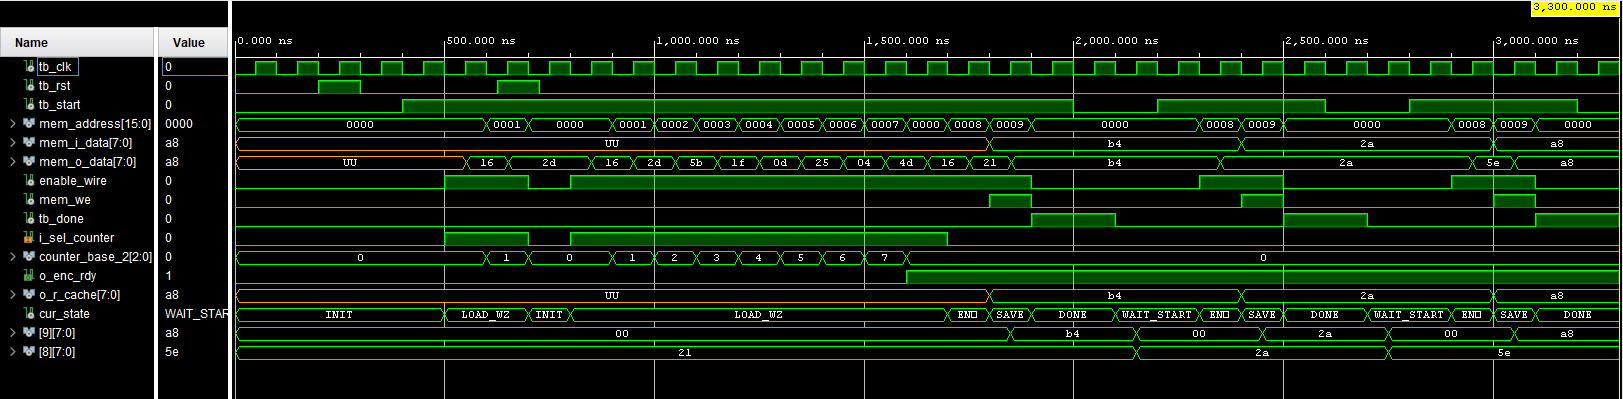
\includegraphics[width=\linewidth]{waveview.png}
  {
    \small
    Working zones: \texttt{[16,2D,5B,1F,0D,25,04,4D]}, Indirizzi: \texttt{[21,2A,5E]}
  }
  \caption{Wave view durante una simulazione}
  \label{fig:wave}
\end{figure}

\section{Conclusioni}

Il design scelto utilizza un registro per working zone, per questo motivo la prima codifica dopo un reset sarà la più lenta, vista la necessità di caricare nei registri gli indirizzi base delle working zones, tuttavia le codifiche successive saranno più veloci usando solo due cicli di clock per la codifica e due per segnalare la fine e attendere un nuovo start.

Un approccio alternativo sarebbe quello di salvare in un registro l'indirizzo da codificare e scorrere tra le working zones confrontando passo passo l'indirizzo con la base delle working zones fermando la codifica se si trova un offset minore di 4 con la base di una working zone, o una volta passate tutte le working zones.

Il secondo approccio richiede un numero minore di registri, che non aumenterebbe se le working zones fossero più numerose e può essere più veloce sulla prima codifica dopo un reset in quanto non richiede una fase di setup iniziale e se l'indirizzo appartiene a una delle prime working zones la codifica termina con pochi cicli di clock.

Tuttavia per le specifiche progettuali il design scelto rientra con ampio margine nei limiti di superficie e, oltre a richiedere meno cicli di clock per codifiche successive, ha il vantaggio di richiedere un numero di cicli di clock costante per la codifica, indipendente dal contenuto della RAM, che potrebbe portare dei vantaggi nella semplicità di utilizzo del componente.

\end{document}